
\label{chap:software-operations_Manager}

\subsection{Adding task to gardeners schedule}

\hrule
\hfill
\vspace{0.5cm}
\label{operation:addTaskGardener}

The manager creates and adds a new task to be added to gardener's schedule.
\begin{description}

\item \textbf{Parameters:} nameTask, taskDescription, room, nameGardener, date,
importance
\item \textbf{Precondition:} The manager is logged in and on the manage gardener
schedule screen
\item \textbf{Post-condition:} A new task has been added to the schedule and the
new task has been assigned to the specified gardener and the manager is
notified that the task has been added.
\item \textbf{Output messages:} The \textbf{manager} will be notified that the
task has been created.

\item \textbf{Triggering:}
\begin{enumerate}
\item From within the manage gardener schedule screen, the \textbf{manger} fills
out the required entries related to the task information like the name of the task or
the date and clicks on the add button.
\item The system then adds the task now to the schedule of the gardener.
\end{enumerate}
\end{description}
\subsubsection{Example of adding a task}
The \textbf{manager} wants to add a watering task to the schedule, so fills out
the textinputfields as shown in the image and then he clicks on the add button.
\begin{figure}[h]
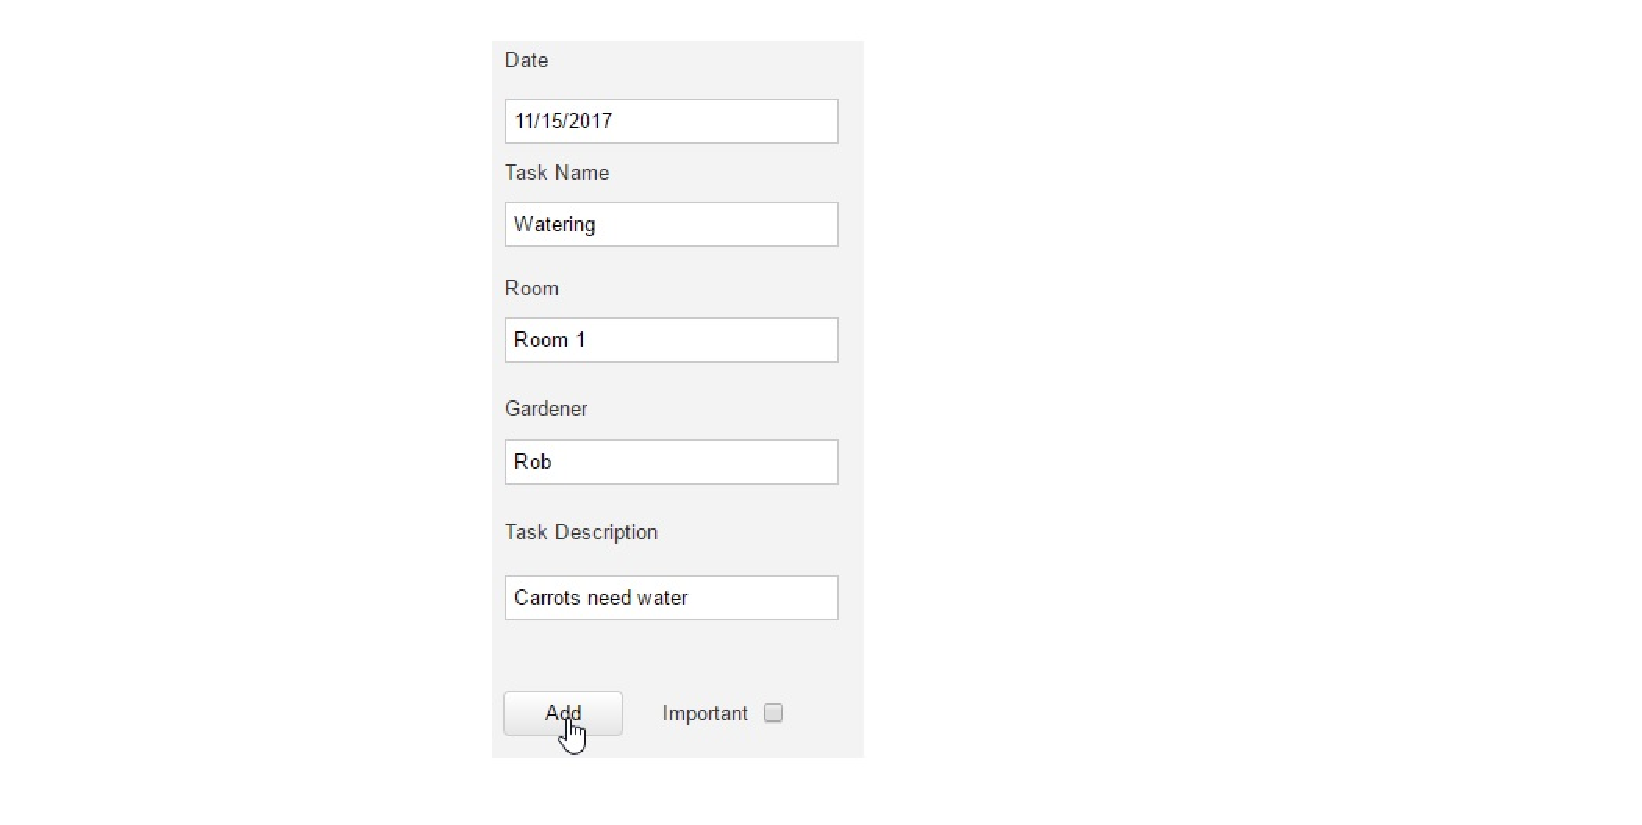
\includegraphics[width=1\textwidth]{images/addingTaskGardener.eps}
\end{figure}

\hfill
\vspace{0.5cm}
\hrule
\break


\subsection{Adding task to technician schedule}

\hrule
\hfill
\vspace{0.5cm}
\label{operation:addTaskTechnichian}

The manager creates and adds a new task to be added to technician's schedule.
\begin{description}

\item \textbf{Parameters:} nameTask, taskDescription, room, nameTechnician,
date, importance
\item \textbf{Precondition:} The manager is logged in and on the manage gardener
schedule screen.
\item \textbf{Post-condition:} A new task has been added to the schedule and the
new task has been assigned to the specified technician and the manager is
notified that the task has been added.
\item \textbf{Output messages:} The \textbf{manager} will be notified that the
task has been created.

\item \textbf{Triggering:}
\begin{enumerate}
\item From within the managa technician schedule screen, the \textbf{manger}
fills out the required entries related to the task information like the name of the task or
the date and clicks on the add button.
\item The \textbf{manager} The system now adds the task to the schedule of the
technician.
\end{enumerate}
\end{description}
\subsubsection{Example of adding a task}
The \textbf{manager} wants to the technician to change sensors, so he fills out
the requied fields and then presses the add button as shown in the image.
\hfill
\vspace{0.5cm}
\hrule

\subsection{Accept a diffrent seed}

\hrule
\hfill
\vspace{0.5cm}

\label{operation:Accept a diffrent seed}

The Manager can accept the request for a new seed which is not already on the
crop inventory table.
\begin{description}
\item \textbf{Parameters:}seedName
\item \textbf{Precondition:} The system is bootedup and the Manager has to be
logged in and be on the Manager request screen.
\item \textbf{Post-condition:} The request has been validated manager
redirected to the manager home screen.
\item \item \textbf{Output messages:} Successfully accepted now add a the seed
to the storage/inventory.
\item \textbf{Triggering:}
\begin{enumerate}
\item \textbf{Manager} presses the green button to validated the request.
\item \textbf{System}redirects the manager to the manager home screen and
displays the output message.

\end{enumerate}
\end{description}

\subsubsection{Example of accepting a request}
\textbf{Manager} accepts by pressing the green button on COCO with the amount
50.\textbf{System} displays a successfully accepted and redirects the manager
to the ma,ager homescreen.
\textbf{Manager}complets the di\ldots\ldots.;;
\hfill
\vspace{0.5cm}
\hrule

\break

\subsection{Accept the request for a new sensor}

\hrule
\hfill
\vspace{0.5cm}

\label{operation:Accept the request for a new sensor}

The Manager can accept a new sensor.
\begin{description}
\item \textbf{Parameters:} /
\item \textbf{Precondition:} The system is bootedup and the Manager has to be
logged in and be on the Manager request screen and a request has to be
available.
\item \textbf{Post-condition:} Validation of the request send to the Technician.
\item \textbf{Output messages:}Successfully allowed to replace the sensor.
\item \textbf{Triggering:}
\begin{enumerate}
\item \textbf{Manager} Presses the green button to validate the request.
\item System sends a message that the sensor can be added to the room to the
technican.
\item \begin{figure}[H]
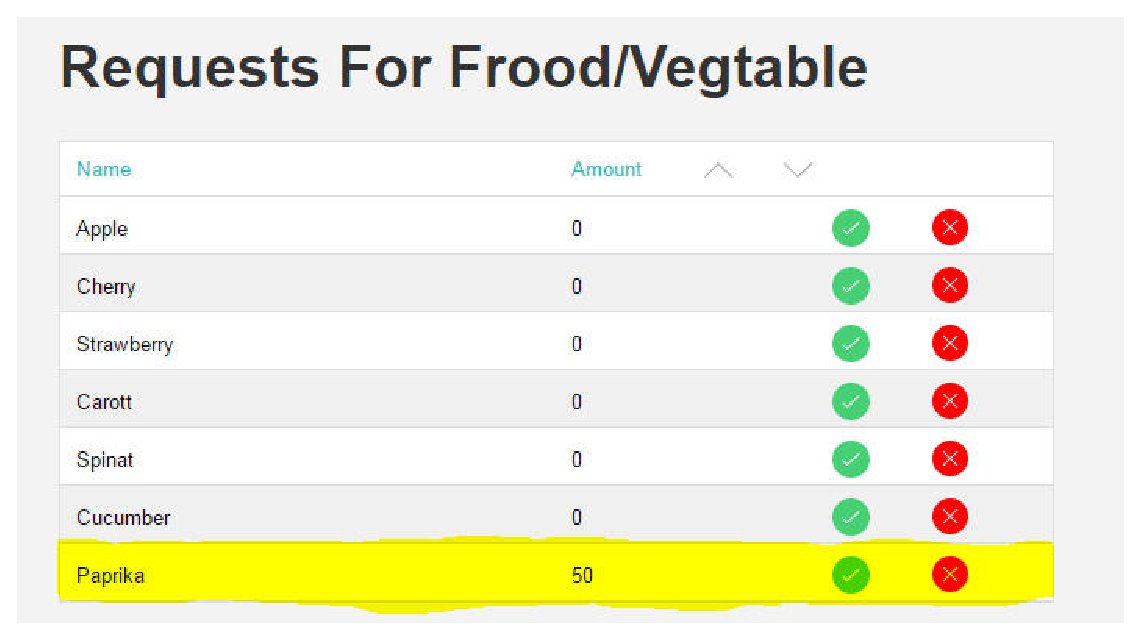
\includegraphics[width=1\textwidth]{images/AcceptRequestedCropManager.eps}
\end{figure}
\end{enumerate}
\end{description}

\subsubsection{Example of accepting a request}
\textbf{Maneger} presses the green button to accept the request from the
Temperature1 Sensor. \textbf{System} sends a validation message to the gardener.
\hfill
\vspace{0.5cm}
\hrule






\break

\subsection{Remove Seed from Inventory}

\hrule
\hfill
\vspace{0.5cm}

\label{operation:RemoveSeed}

The manager can remove a given kind of seed completly.
\begin{description}

\item \textbf{Parameters:} NameSeed, Amount
\item \textbf{Precondition:} The system is bootedup and manager has to be
logged in and be on the manager request screen.
\item \textbf{Post-condition:} Request table has been updated with the removed
seed.
\item \textbf{Output messages:} Successfully removed item.
\item \textbf{Triggering:}
\begin{enumerate}
\item \textbf{Manager} presses the red button on the crops inventory table.
\item \begin{figure}[H]
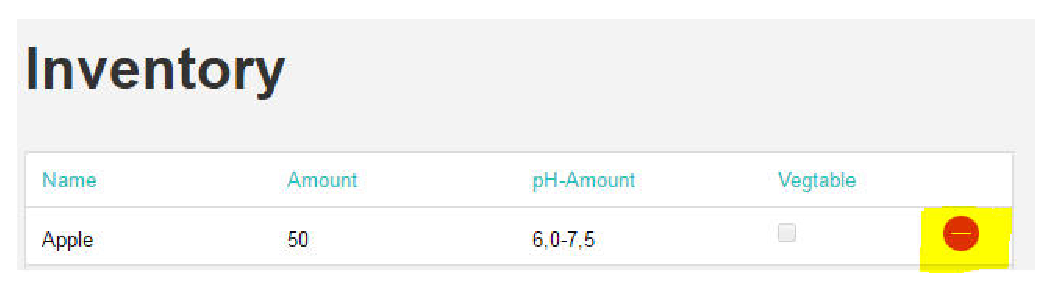
\includegraphics[width=1\textwidth]{images/RemoveSeedFromInventory.eps}
\end{figure}
\item System removes the seeds from the seed inventory on the manager and
gardener screen.
\end{enumerate}
\end{description}

\subsubsection{Example of removing crops}
\textbf{Manager} removes the seed by pressing the red button. The System
updates the changes on the manager request screen and Gardener screen.
\hfill
\vspace{0.5cm}
\hrule

\break


\subsection{Sort request seed by amount ascending order}

\hrule
\hfill
\vspace{0.5cm}

\label{operation:sortSeedRequest}

The manager can sort the seed which are requested by ascanding order.
\begin{description}

\item \textbf{Parameters:} /
\item \textbf{Precondition:} The system is bootedup and manager has to be
logged in and be on the manager request screen.
\item \textbf{Post-condition:} Request seed table has been ordered in ascanding
order.

\item \textbf{Output messages:} none
\item \textbf{Triggering:}
\begin{enumerate}
\item \textbf{Manager} presses the top arrow.
\item System sorts the list by amount value by ascending order.
\begin{figure}[H]
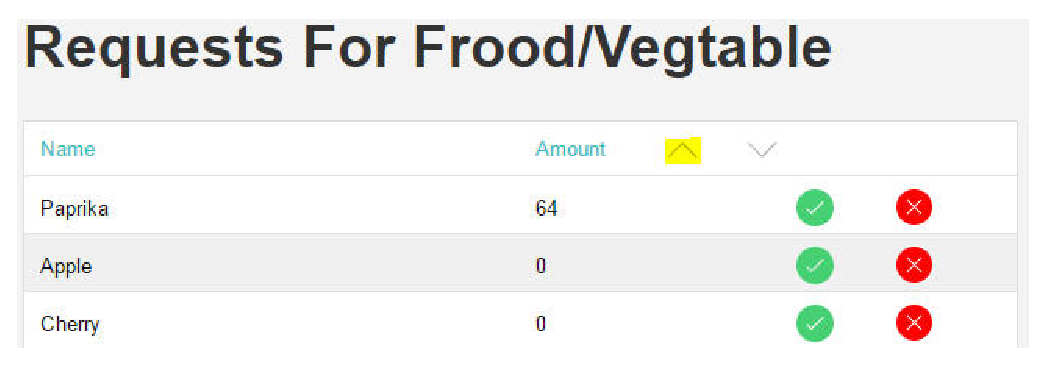
\includegraphics[width=1\textwidth]{images/RequestByAscendingOrderManager.eps}
\end{figure}
\end{enumerate}
\end{description}

\subsubsection{Example of removing crops}
\textbf{Manager} presses the arraw on the request seed table. System sorts the
the table by amount in ascending order.

\hfill
\vspace{0.5cm}
\hrule

\break

\subsection{Add seed to the inventory request Gardener}

\hrule
\hfill
\vspace{0.5cm}

\label{operation:Add a diffrent seed request Gardener}

The Manager can add a new seed to the inventory.
\begin{description}
\item
\textbf{Parameters:}Name,Amount,ph-Amount,Vegtable(boolean),TemperaturePreference
\item \textbf{Precondition:} The system is bootedup and the Manager has to be
logged in and be on the Manager screen and a request has to be accepted by the
manager.
\item \textbf{Post-condition:} The invenotry has been updated by adding the
attributes to the table.
\item 
\item \item \textbf{Output messages:} Successfully accepted the request
\item \textbf{Triggering:}
\begin{enumerate}
\item \textbf{Manager} complets the formula and presses the add button.
\begin{figure}[H]
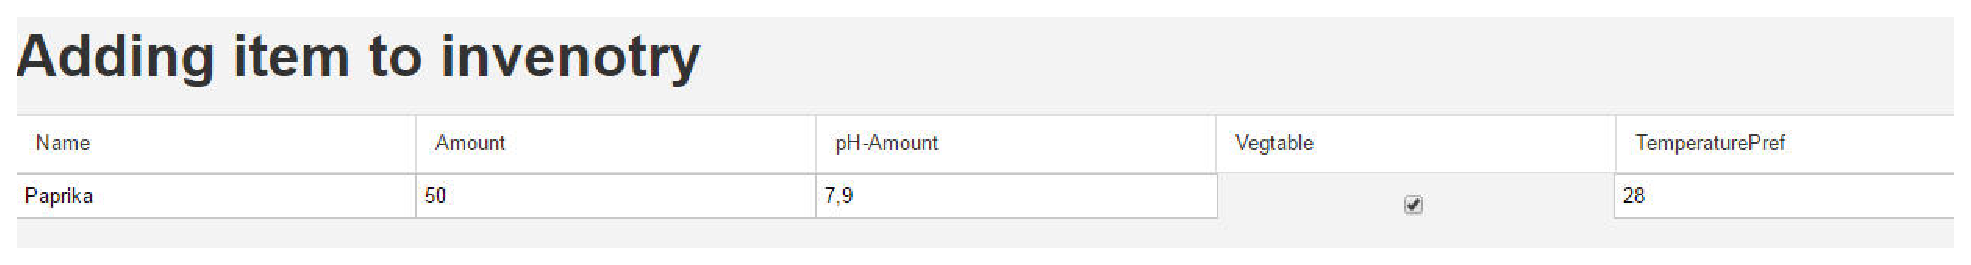
\includegraphics[width=1\textwidth]{images/AddingSeedToTheInventoryManager.eps}
\end{figure}
\item \textbf{System} shows a pop up of the entered values.
\begin{figure}[H]
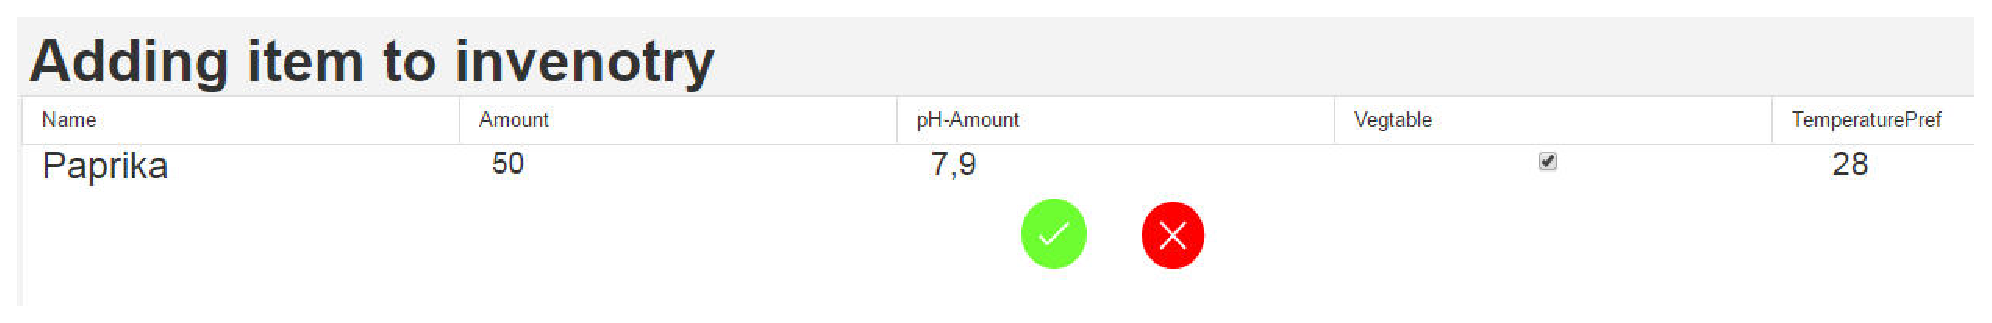
\includegraphics[width=1\textwidth]{images/AddingSeedToTheInventoryPopUp.eps}
\end{figure}
\item \textbf{Manager} accepts the pop up request.
\item \textbf{System} displays a message of success and adds the values to the
inventory crop table.

\end{enumerate}
\end{description}

\subsubsection{Example of adding a non exisiting seed to the storage}
\textbf{Manager} complets the given inputs text field with the
Name: Coconut and amount 50 and ph value 9 and Vegtable false
(not coching the crop field) and temperature preference : 34. \textbf{System}
displays a pop up  what the user has entered in this case Coconut 50 9 (false)
and 34.Manager accepts the pop up by pressing the green button. System updates
the crop inventory table by adding the input values from the manager to the
table.
\hfill
\vspace{0.5cm}
\hrule

\break
\subsection{Refill storage of seeds}

\hrule
\hfill
\vspace{0.5cm}

\label{operation:Refill storage System request}

The Manager accept to refill the storage of seed requested by the system.
\begin{description}
\item
\textbf{Parameters:}Name,Amount,ph-Amount,Vegtable(boolean),TemperaturePreference
\item \textbf{Precondition:} The system is bootedup and the Manager has to be
logged in and be on the Manager request screen and there needs to be a request
from the system for seeds.
\item \textbf{Post-condition:} The inventory storage of the requested seed has
been updated.
\item 
\item \item \textbf{Output messages:} Successfully refilled the storage
\item \textbf{Triggering:}
\begin{enumerate}
\item \textbf{Manager} presses the green button on the request seed table.
\item \textbf{System} displays a message that the storage was sucessfully
refilled.
\end{enumerate}
\end{description}

\subsubsection{Example of accepting a request}
\textbf{Manager} Presses on the green button from Apple where the amount of
requested seeds is 20. \textbf{System} updates the inventory by adding 20 to the
apple seeds amount and displays the message: Successfully refilled storage.
\hfill
\vspace{0.5cm}
\hrule



\subsection{Add new security camera}
\hrule
\hfill
\vspace{0.5cm}
\label{operation:Add new security camera}

The manager can add a new security camera to the system.

\begin{description}

\item \textbf{Parameters:} ID, Description, Indoor
\item \textbf{Precondition:} The system is bootedup and the Manager has to be
logged in and be on the Settings pop-up screen.
\item \textbf{Post-condition:} The new security camera has been added to the security camera database.
\item \textbf{Triggering:}
\begin{enumerate}

\item \textbf{Manager} fills in the different input text fields and presses
the add security camera button.

\end{enumerate}
\end{description}

\subsubsection{Example of adding a new security camera}
\textbf{Manager} fills in the identifier (ID = 10), the description (Description = 'Camera 10 Entrance') and if the camera is indoor (Indoor = true). 
Now the \textbf{Manager} presses the 'Add Camera' button to add a new entry into the security camera database.
\hfill
\vspace{0.5cm}
\hrule

\break

\subsection{Delete security camera}
\hrule
\hfill
\vspace{0.5cm}
\label{operation:Delete security camera}

The manager can delete a security camera from the system.

\begin{description}

\item \textbf{Parameters:} ID
\item \textbf{Precondition:} The system is bootedup and the Manager has to be
logged in and be on the Settings pop-up screen.
\item \textbf{Post-condition:} The choosen security camera has been removed from the security camera database.
\item \textbf{Triggering:}
\begin{enumerate}

\item \textbf{Manager} clicks on the remove button on the security camera to be deleted.

\end{enumerate}
\end{description}

\subsubsection{Example of deleting security camera}
The \textbf{Manager} looks for the needless security camera and click on the red remove button to delete the security camera from the system.
\hfill
\vspace{0.5cm}
\hrule





\subsection{Show single security camera view}
\hrule
\hfill
\vspace{0.5cm}
\label{operation:Show single security camera view}

The manager can choose a single security camera to be viewed instead of the 4 view perspective.

\begin{description}

\item \textbf{Parameters:} ID
\item \textbf{Precondition:} The system is bootedup and the Manager has to be
logged in and be on the Security Camera pop-up screen.
\item \textbf{Post-condition:} The choosen security camera is shown in fullscreen.
\item \textbf{Triggering:}
\begin{enumerate}

\item \textbf{Manager} selects a security camera from the select list and presses 'View Camera'.

\end{enumerate}
\end{description}

\subsubsection{Example of showing a single security camera view}
The \textbf{Manager} chooses a security camera from the select list which he wants the view in fullscreen. To change the view  the \textbf{Manager} clicks on the button 'View Camera'.
\hfill
\vspace{0.5cm}
\hrule


\break

\subsection{Show multiple security camera view}
\hrule
\hfill
\vspace{0.5cm}
\label{operation:Show multiple security camera view}

The manager can choose to view 4 security cameras at the same time.

\begin{description}

\item \textbf{Parameters:} 
\item \textbf{Precondition:} The system is bootedup and the Manager has to be
logged in and be on the Security Camera pop-up screen.
\item \textbf{Post-condition:} The security camera screen now shows 4 views of up to 4 different security cameras.
\item \textbf{Triggering:}
\begin{enumerate}

\item \textbf{Manager} clicks on the button '4 Camera View'.

\end{enumerate}
\end{description}

\subsubsection{Example of showing a multiple security camera view}
The \textbf{Manager} clicks on the '4 Camera View' button to display more security cameras at the same time.
\hfill
\vspace{0.5cm}
\hrule




\subsection{Add a new crop to the CropsDatabase}
\hrule
\hfill
\vspace{0.5cm}
\label{operation:Add a new crop the CropsDatabase}

The manager can add a new crops to the crops database.

\begin{description}

\item \textbf{Parameters:} ID, DatePlanted, DateHarvested, Room, Plant, Weight, NumberOfPlants
\item \textbf{Precondition:} The system is bootedup and the Manager has to be
logged in and be on the Crops Manager pop-up screen.
\item \textbf{Post-condition:} The new crop is added to the crops database.
\item \textbf{Triggering:}
\begin{enumerate}

\item \textbf{Manager} fills out the input text fields and clicks on the button 'Add new Crop'.

\end{enumerate}
\end{description}

\subsubsection{Example of adding a new crop to the CropsDatabase}
The \textbf{Manager} fills out the input text fields with the corresponding data and then adds a new crops to the database by pressing the 'Add new crop' button.
\hfill
\vspace{0.5cm}
\hrule


\break

\subsection{Delete a crop from the CropsDatabase}
\hrule
\hfill
\vspace{0.5cm}
\label{operation:Delete a crop from the CropsDatabase}

The manager can delete a crop from the crops database.

\begin{description}

\item \textbf{Parameters:} ID
\item \textbf{Precondition:} The system is bootedup and the Manager has to be
logged in and be on the Crops Manager pop-up screen.
\item \textbf{Post-condition:} The choosen crop is deleted from the crops database.
\item \textbf{Triggering:}
\begin{enumerate}

\item \textbf{Manager} clicks on the remove button next to the crop to be deleted from the crops database.

\end{enumerate}
\end{description}

\subsubsection{Example of deleting a crop from the CropsDatabase}
The \textbf{Manager} looks for the crops he wants to remove from the crops database. And to remove the crop, the \textbf{Manager} clicks on the red remove button next to the crop.
\hfill
\vspace{0.5cm}
\hrule




\subsection{Add a new room}
\hrule
\hfill
\vspace{0.5cm}
\label{operation:Add a new room}

The Manager can add a new room to the room database.

\begin{description}

\item \textbf{Parameters:} ID, RoomName, Width, Length, SoilHeight
\item \textbf{Precondition:} The system is bootedup and the Manager has to be
logged in and be on the Settings pop-up screen.
\item \textbf{Post-condition:} The new room has been added to the room database.
\item \textbf{Triggering:}
\begin{enumerate}

\item \textbf{Manager} fills out the input text fields and clicks on the 'Add Room' button.

\end{enumerate}
\end{description}

\subsubsection{Example of adding a new room}
The \textbf{Manager} fills in the identifier (ID = 2), the room name (RoomName = 'Room 2'), the width (Width = 5), the length (Length = 3) and the soil height (SoilHeight = 0,5).
Now the \textbf{Manager} clicks on the 'Add Room' button to add a new room to the room database.
\hfill
\vspace{0.5cm}
\hrule


\break

\subsection{Delete a room}
\hrule
\hfill
\vspace{0.5cm}
\label{operation:Delete a room}

The Manager can delete a room from the room database.

\begin{description}

\item \textbf{Parameters:} ID
\item \textbf{Precondition:} The system is bootedup and the Manager has to be
logged in and be on the Settings pop-up screen.
\item \textbf{Post-condition:} The selected room has been removed from the room database.
\item \textbf{Triggering:}
\begin{enumerate}

\item \textbf{Manager} clicks on the red remove button next to the room to be deleted.

\end{enumerate}
\end{description}

\subsubsection{Example of deleting a room}
The \textbf{Manager} looks for the room that is no longer needed and clicks on the red remove button next to the entry.
\hfill
\vspace{0.5cm}
\hrule

 



